
\documentclass{article}
\usepackage[utf8]{inputenc}
\usepackage{graphicx}
\usepackage{geometry}
 \geometry{
	 a4paper,
	 total={170mm,257mm},
	 left=20mm,
 	top=20mm,
 } 
 
\title{DU@UP ObjectSensor and Mobile Navigation \\
The Inevitables
}

\author{  
            Peter Rayner\\
            Dawie Pritchard\\
            Drew Langley\\
            Hendrik Jan van der Merwe\\
            Lyle Nel\\
        }


\begin{document}

\maketitle

\includegraphics[width=20cm,height=11cm,keepaspectratio]{group.JPG}

\newpage

\tableofcontents

\newpage


\section{High level description}
A mobile navigation application that allows for the independent navigation of persons with visual disabilities. The combination of technologies, navigation systems and low tech devices will help students navigate their way on campus safely and successfully. 

\subsection{Software and Hardware Characteristics:}
The mobile application should make use of bluetooth tags that enables the localisation and distance of an obstacle. The bluetooth transmitters communicate with a students mobile device to send information of the students position and determine distance from the obstacle. The creation of obstacle sensors will reliably detect when a student is getting too close to an obstacle. The application should also include a short series of audible beeps to notify a student of an impending obstacle. The application should work indoors and outdoors at UP Route speech navigation. The software should adhere to all UP policies and should be free of any malicious code.

\subsection{System requirements:}
The application should be developed to be downloaded and installed on devices from Apple's App Store or Google's Play Store.
It should comply with the most recent web accessibility guidelines and should also be percievable, operable, understandable and robust.
The obstacle sensors should be enabled via bluetooth.
The application should work cross platform (iOS, Android, Windows, Mobile Web), Device formats would include phones and tablets. Navigation should work through the use of WiFi Access point data.

\subsection{Possible Project Name}
NavUP

\section{Proposed Solution}

\subsection{Technologies}
\begin{itemize}
	\item J2EE
	\item JDBC
	\item JPA
	\item Wildfly 10
	\item MongoDB
\end{itemize}
Note that during the course of the development some technologies may be included/ excluded based on the needs of the system.
\subsection{Deployment Diagram}
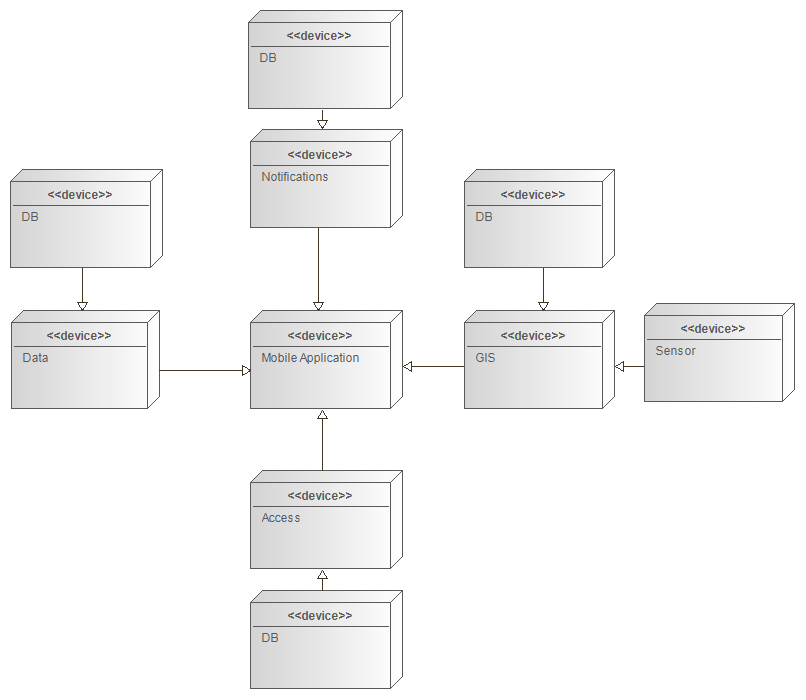
\includegraphics[width=20cm,height=11cm,keepaspectratio]{dd1.png} \\

\subsubsection{Description}
We intend to use a microservices architecture which provides loose coupling and high cohesion between a set of individually created modules. There will in essence be four modules, where each module can have an independent architecture if necessary. The modules will be data, notifications, GIS, Access. The mobile application will be used to find locations and navigate to them, this will include the audible beeps, the rest of the modules will be used to gather information about locations on campus, as well as coordinates for these locations(indoors and outdoors).
\section{Development Methodology}
We will be using the Agile Scrum Methodology. By making a backlog of work to be done and by completing deadlines in short iterations or sprints. We will meet daily by making use of  Slack Messaging Platform to discuss the progress as well as obstacles and how to overcome these obstacles by getting input from each member. We will also define when these deadlines are and make sure we keep to the schedule. We will meet everytime we are done with a deadline to reflect on the work done. \\ \\
At each deadline or meeting we will make sure we meet with the client to make sure that they are kept up to date with our progress. We will also meet with the client when there are concerns or obstacles to overcome to make sure the client knows about these obstacles. The client will be kept up to date each week with the progress of the project.
\section{Cost Analysis}
The estimated cost to develop both software and hardware to be determined by UP Department of Computer Science.

\section{Risk Analysis}
\subsection{Privacy}
The Protection of Personal Information Act, No 4 of 2013, is applicable in this project due to data collection of personal information. We caution that due diligence be exercised when deploying the system within a UP campus. The act requires that the data subject gives consent. Compliance with the act has additional implications for security, custody of the collected data and how it may be processed.

\subsection{Security}
There are security concerns regarding the use of  the sensors that are involved. Precautions will have to be taken to ensure that students/lecturers' information and access to these sensors are limited to only those who need access.


\section{Team Details}
\subsection{Dawie Pritchard}
Final Year BIS multimedia student with only computer science subjects remaining.
\textbf{Skills:}
University level skills of:
\begin{itemize}
 	\item Human Computer Interaction
 	\item Trends, Visual Design 
 	\item Multimedia
 	\item Computer Science
\end {itemize}
\textbf{Technologies known:}
\begin{itemize}
	\item C
 	\item C++
 	\item C-Sharp
 	\item CSS
 	\item Bootstrap
 	\item Java
 	\item Python
 	\item Javascript / AngularJS / ExpressJS / NodeJS / JQUERY
 	\item MongoDB / NoSQL
 	\item Php
 	\item SQL
 	\item HTML5
 	\item XML
 \end{itemize}
\textbf{Stengths:} 
\begin{itemize}
	\item Front-End
	\item Back-End development
\end{itemize}

\newpage
\subsection {Peter Rayner}

\textbf{Front-end developer with knowledge of:}
\begin{itemize}
 	\item Artifical Intelligence
 	\item Data structures 
 	\item Website design 
 	\item Databases and human computer interaction(user experience)
 \end{itemize}
\textbf{Technologies known:}
\begin{itemize}
	\item C++ 
	\item C 
	\item C\# 
	\item Java 
	\item JavaScript 
	\item Python 
	\item Assembly 
	\item AngularJS  
	\item Bootstrap
 \end{itemize}
\textbf{Previous industry experience:}\\
Working at Barclays CIB in big data and analytics.
\\
\newpage
\subsection {Hendrik Jan van der Merwe} 
\textbf{University level knowledge of:}
\begin{itemize}
 	\item Data structures
 	\item Databases
 	\item Human Computer Interaction focussing on User Experience
 	\item System Design
\end{itemize}
\textbf{Technologies known:}
\begin{itemize}
	\item C++
	\item C\#
	\item Java
	\item SQL / MySQL
	\item MongoDB
	\item PHP
	\item JavaScript / AJAX / JQuery / NodeJS / ExpressJS
	\item HTML / CSS / Bootstrap
	\item XML
\end{itemize}
\textbf{Strengths:}
\begin{itemize}
	\item Database Design
	\item Backend Development
\end{itemize}

\newpage
\subsection {Lyle Nel}
\textbf{Qualifications:} \\
I hold a BTEC in software engineering, which included project management as part of the curriculum.
I also hold a BSc in Computer Systems, with relevant subjects such as Software Engineering, Operations management, Knowledge management, Professional development, and Artificial intelligence.\\ \\
\textbf{Digital electronics:} \\
I have worked with Atmel and ARM microprocessors as well as on the arduino platform. In addition I am familiar with most of the common components of a digital circuit including 7400 series and 4000 series integrated circuits. \\ \\
\textbf{Computer Hardware:} \\
I am familiar with all standard consumer hardware and some server hardware. I maintain my own server cluster at home for running experiment. \\ \\
\textbf{Artificial intelligence} \\
I am most experienced in genetic algorithms and I am the author of an open source project that cracks passwords using genetic algorithms. The was one of the top 3 trending projects on github and hackernews a while back. See https://github.com/lyle-nel/siga. In general I am very comfortable with solving problems within the domain of AI. \\ \\
\textbf{Languages} \\
C, C++ including the new C++11, C++14 and C++17 ISO standards, Bash, Python, Javascript, Java, Lisp and Prolog. The language that I am most comfortable with is C++. When I conduct experiment on large datasets I use a mixture between C++, Python and Bash. \\ \\
\textbf{Platforms} \\
I do all of my work in a Linux environment.

\newpage
\subsection {Drew Langley}
Third year BIS Multimedia student with experience in UX and HCI, animation and 3D modelling, Web design and databases as well as proficiency in programming. I am currently studying networks, software engineering and Artificial Intelligence. \\ \\
\textbf{Technologies known:}
\begin{itemize}
	\item HTML
	\item CSS 
	\item JS / AngularJS / NodeJS / JQuery 
	\item PHP 
	\item SQL
	\item MongoDB
	\item Java 
	\item C++ 
	\item C 
	\item C\# 
	\item Python 
	\item Assembly
\end{itemize}
\textbf{Experience:} \\
Designed and developed www.ugandaprohunts.com

\textbf{Stengths:} 
\begin{itemize}
	\item Front-End
	\item Back-End development
\end{itemize}

\end{document}
